\documentclass[../DoAn.tex]{subfiles}
\begin{document}

Chương này trình bày chi tiết quá trình thực nghiệm, bao gồm việc huấn luyện các mô hình SVM và CNN và kiểm tra hiệu suất của chúng trên tập dữ liệu MNIST.

\section{Huấn luyện mô hình}

Quá trình huấn luyện hai mô hình SVM và CNN được thực thi thông qua các hàm \texttt{run\_svm\_project()} và \texttt{run\_cnn\_project()} trong file \texttt{main.py}. Kết quả độ chính xác và ma trận nhầm lẫn chi tiết được hiển thị trực tiếp trên terminal và đã được tổng hợp trong Chương 4.\\

\section{Kiểm tra mô hình}

Để đánh giá hiệu suất của hai mô hình, em đã thiết kế một giao diện ứng dụng cho phép lấy ngẫu nhiên các ảnh chữ số dựa trên nhãn được chọn trước để tiến hành kiểm tra.

\begin{figure}[H]
    \centering
    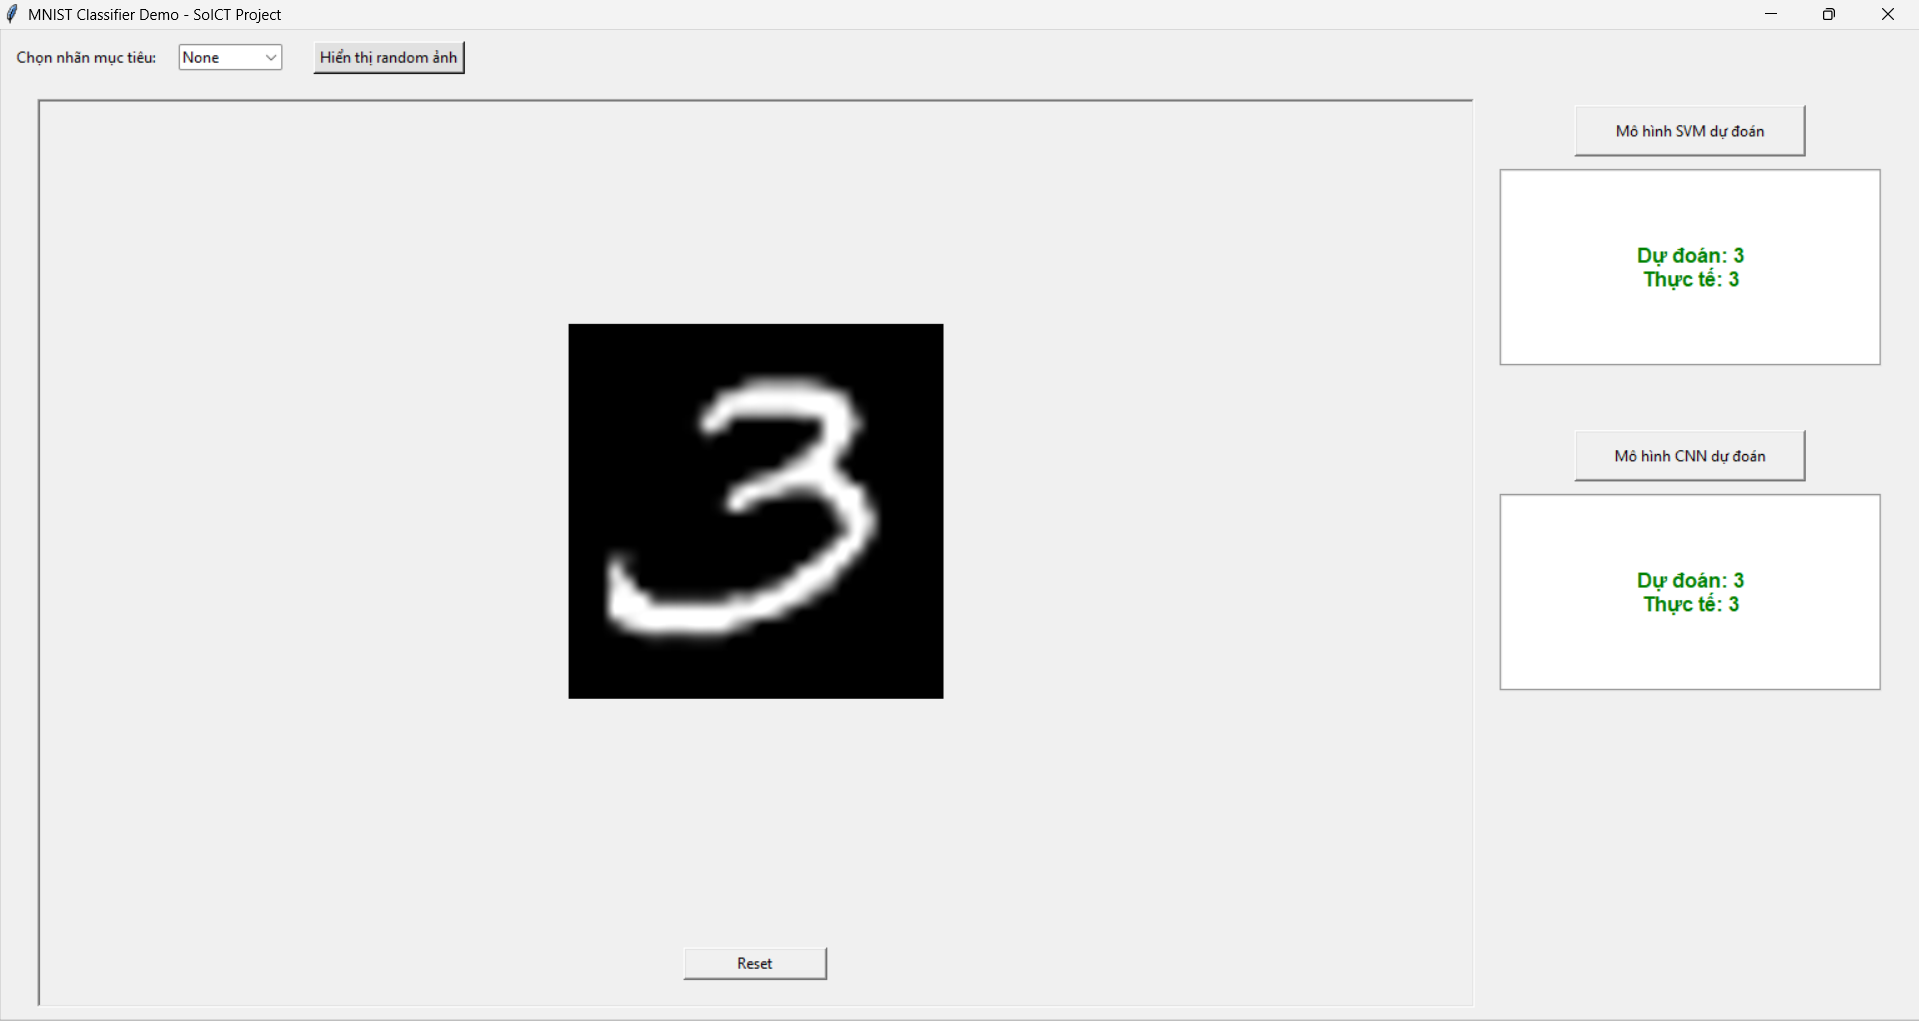
\includegraphics[trim={10pt 20pt 10pt 20pt}, clip,width=1.0\textwidth]{../Hinh_ve/app1.png}
    \caption{SVM và CNN đều nhận diện đúng số 3}
    \label{fig:app1}
\end{figure}

Hình 5.2 minh họa trường hợp mô hình SVM nhận diện sai chữ số 7 thành số 2, nhưng mô hình CNN vẫn nhận diện chính xác, minh chứng cho khả năng học đặc trưng hình học mạnh mẽ hơn của CNN.

\begin{figure}[H]
    \centering
    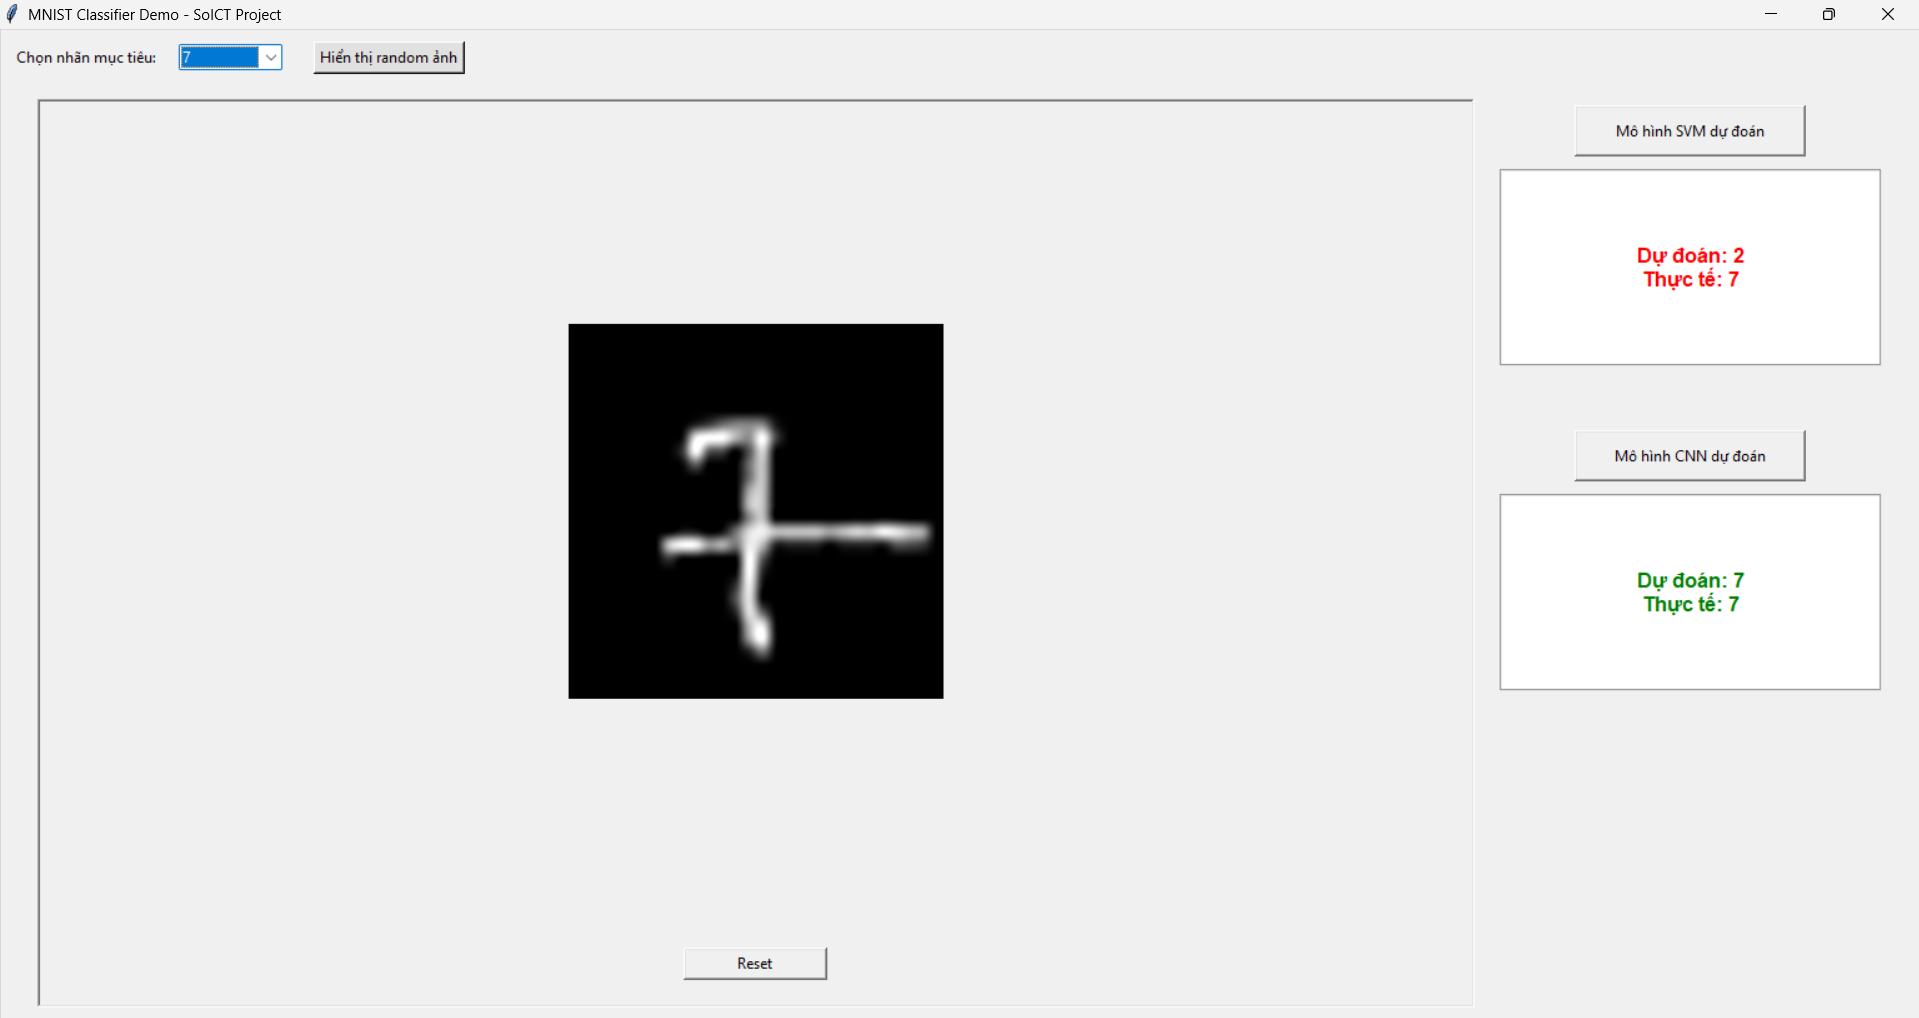
\includegraphics[trim={10pt 20pt 10pt 20pt}, clip,width=1.0\textwidth]{../Hinh_ve/app2.png}
    \caption{SVM nhận diện sai số 7 thành số 2, CNN nhận diện đúng}
    \label{fig:app2}
\end{figure}

\end{document}